%Language: LaTeX
%Script: Florida.tex
%Des: Is Florida warmer?

\documentclass[12pt]{article}

%\date{Oct, 2021}

% Language setting
% Replace `english' with e.g. `spanish' to change the document language
\usepackage[english]{babel}

% Set page size and margins
% Replace `letterpaper' with`a4paper' for UK/EU standard size
\usepackage[letterpaper,top=2cm,bottom=2cm,left=3cm,right=3cm,marginparwidth=1.75cm]{geometry}

% Useful packages
\usepackage{amsmath}
\usepackage{graphicx}
\graphicspath{{../writeup/}}
\usepackage[colorlinks=true, allcolors=blue]{hyperref}
\usepackage{float}

\title{Is Florida getting warmer?}
\author{Congjia Chen (Congjia.Chen21@imperial.ac.uk)}

\begin{document}
\maketitle

\begin{abstract}
The climate change is a crtical issue wouldwide. By examining the annual temperature data set from Key West in Florida, USA for the 20th century, we use the correlation coefficients between temperature and time to see if Florida is getting warmer? However, because measurements of climatic variables in successive time-points in a time series (successive seconds, minutes, hours, months, years, etc.) are not independent, we can’t use the standard p-value calculated for a correlation coefficient. Therefore we will use a permutation analysis instead, by generating a distribution of random correlation coefficients and compare our observed coefficient with this random distribution. As a result, the results showed a weak but significant.
correlation between temperature of one year and its successive year. 

\end{abstract}

\section{Introduction}

Is Florida getting warmer? we will examine it using a data set from Florida, USA for the 20th century. However, because measurements of climatic variables in successive time-points in a time series (successive seconds, minutes, hours, months, years, etc.) are not independent, we can’t use the standard p-value calculated for a correlation coefficient. Therefore we will use a permutation analysis instead, by generating a distribution of random correlation coefficients and compare our observed coefficient with this random distribution. As a result,  the results showed a weak but significant
correlation between temperature of one year and its successive year. We hypothesis that the temperatures have a positive correlation with the successive year.

\section{Materials and Methods}

\subsection{Raw Data}
The data consists of two columns: one is temperatures and another is years (grows successively from 1901 to 2000). The raw data file of temperatures and years is named as \href{https://github.com/nedchen2/CMEECourseWork/blob/master/week3/data/KeyWestAnnualMeanTemperature.RData}{KeyWestAnnualMeanTemperature.Rdata}

\subsection{Correlation Coefficients}
The correlation coefficient is a measure that determines the degree to which the movement of two different variables is associated. The Pearson product-moment correlation is used to measure the linear relationship between the temperatures and years. R function (cor())  was used to calculate Pearson's correlation coefficient between temperatures and years in this report.

\subsection{Estimation of \texorpdfstring{$\mathit{p}$}{}-value}
In order to estimate \textit{p}-value, values of temperature were rearranged randomly to years. After reshuffling, Pearson's correlation coefficient were calculated and stored. Repeat this calculation 10,000 times, the approximate \textit{p}-value could be represented by the fraction of the random correlation coefficients whose absolute value were greater than the observed one .

\section{Results}

\subsection{Coefficient Efficient distribution}
After repeating 10,000 times, we have 10001 correlation coefficients (10000 random and 1 raw). See density distribution below \ref{fig:Density_plot}:
The blue dash line demonstrated the correlation coefficients of the raw data set. The 10000 random correlation coefficient shows random distribution. Approximately no random correlation coefficients are bigger than the raw one. The correlation coefficient of the raw data set is 0.53317.
\begin{figure}[H]
\centering
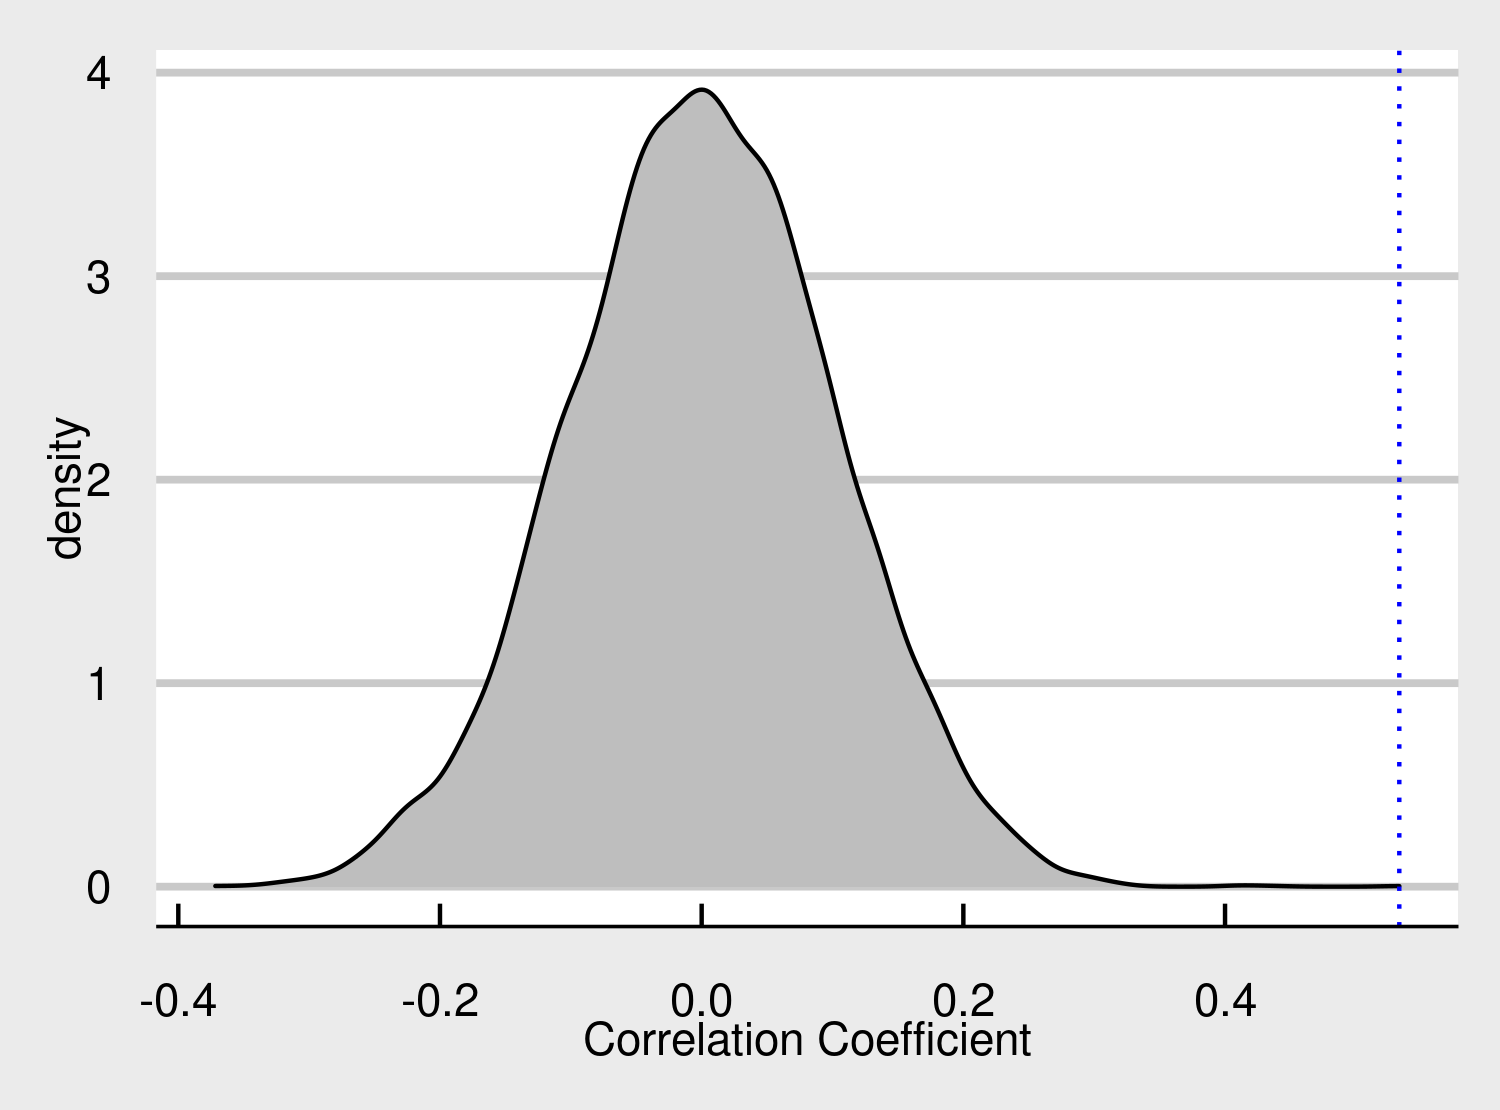
\includegraphics[width=0.7\textwidth]{Density_plot.png}
\caption{\label{fig:Density_plot}The Density plot of Correlation Coefficient}
\end{figure}

\subsection{Estimation of \texorpdfstring{$\mathit{p}$}{}-value}
The approximate \textit{p}-value could be represented by the fraction of the random correlation coefficients whose absolute value were greater than the observed one. The fraction is 0.00000.

\section{Discussion}

\subsection{Coefficient efficient distribution}
The correlation coefficient is 0.53317, showing that there is a relatively weak positive correlation between the temperatures of one year and its successive year. In terms of the statistical significance, we use a permutation analysis, by generating a distribution of random correlation coefficients and compare our observed coefficient with this random distribution. Fraction of the random correlation coefficients whose absolute value were greater than the observed one is 0, indicating the significance statistically.

\section{Conclusion}
In conclusion, a significant positive correlation coefficient was found between temperatures and successive years in Florida( 20th Century), indicating the Florida is getting warmer continuously.

\section{Supplement}
  All codes can be found in Florida.R, please visit the code in \href{https://github.com/nedchen2/CMEECourseWork/blob/master/week3/code/Florida.R}{my repository}.
\end{document}